\documentclass{article}

\usepackage{graphicx}
\usepackage{tikz}
\usepackage{tikzsymbols}
\usetikzlibrary{calc,patterns,shapes.geometric}
\pagestyle{empty}
\usepackage[margin=0pt]{geometry}
\geometry{papersize={14in,12in}}

\def\centerarc[#1](#2)(#3:#4:#5){\draw[#1] ($(#2)+({#5*cos(#3)},{#5*sin(#3)})$) arc (#3:#4:#5);}

\begin{document}
	\begin{figure}
		\centering
		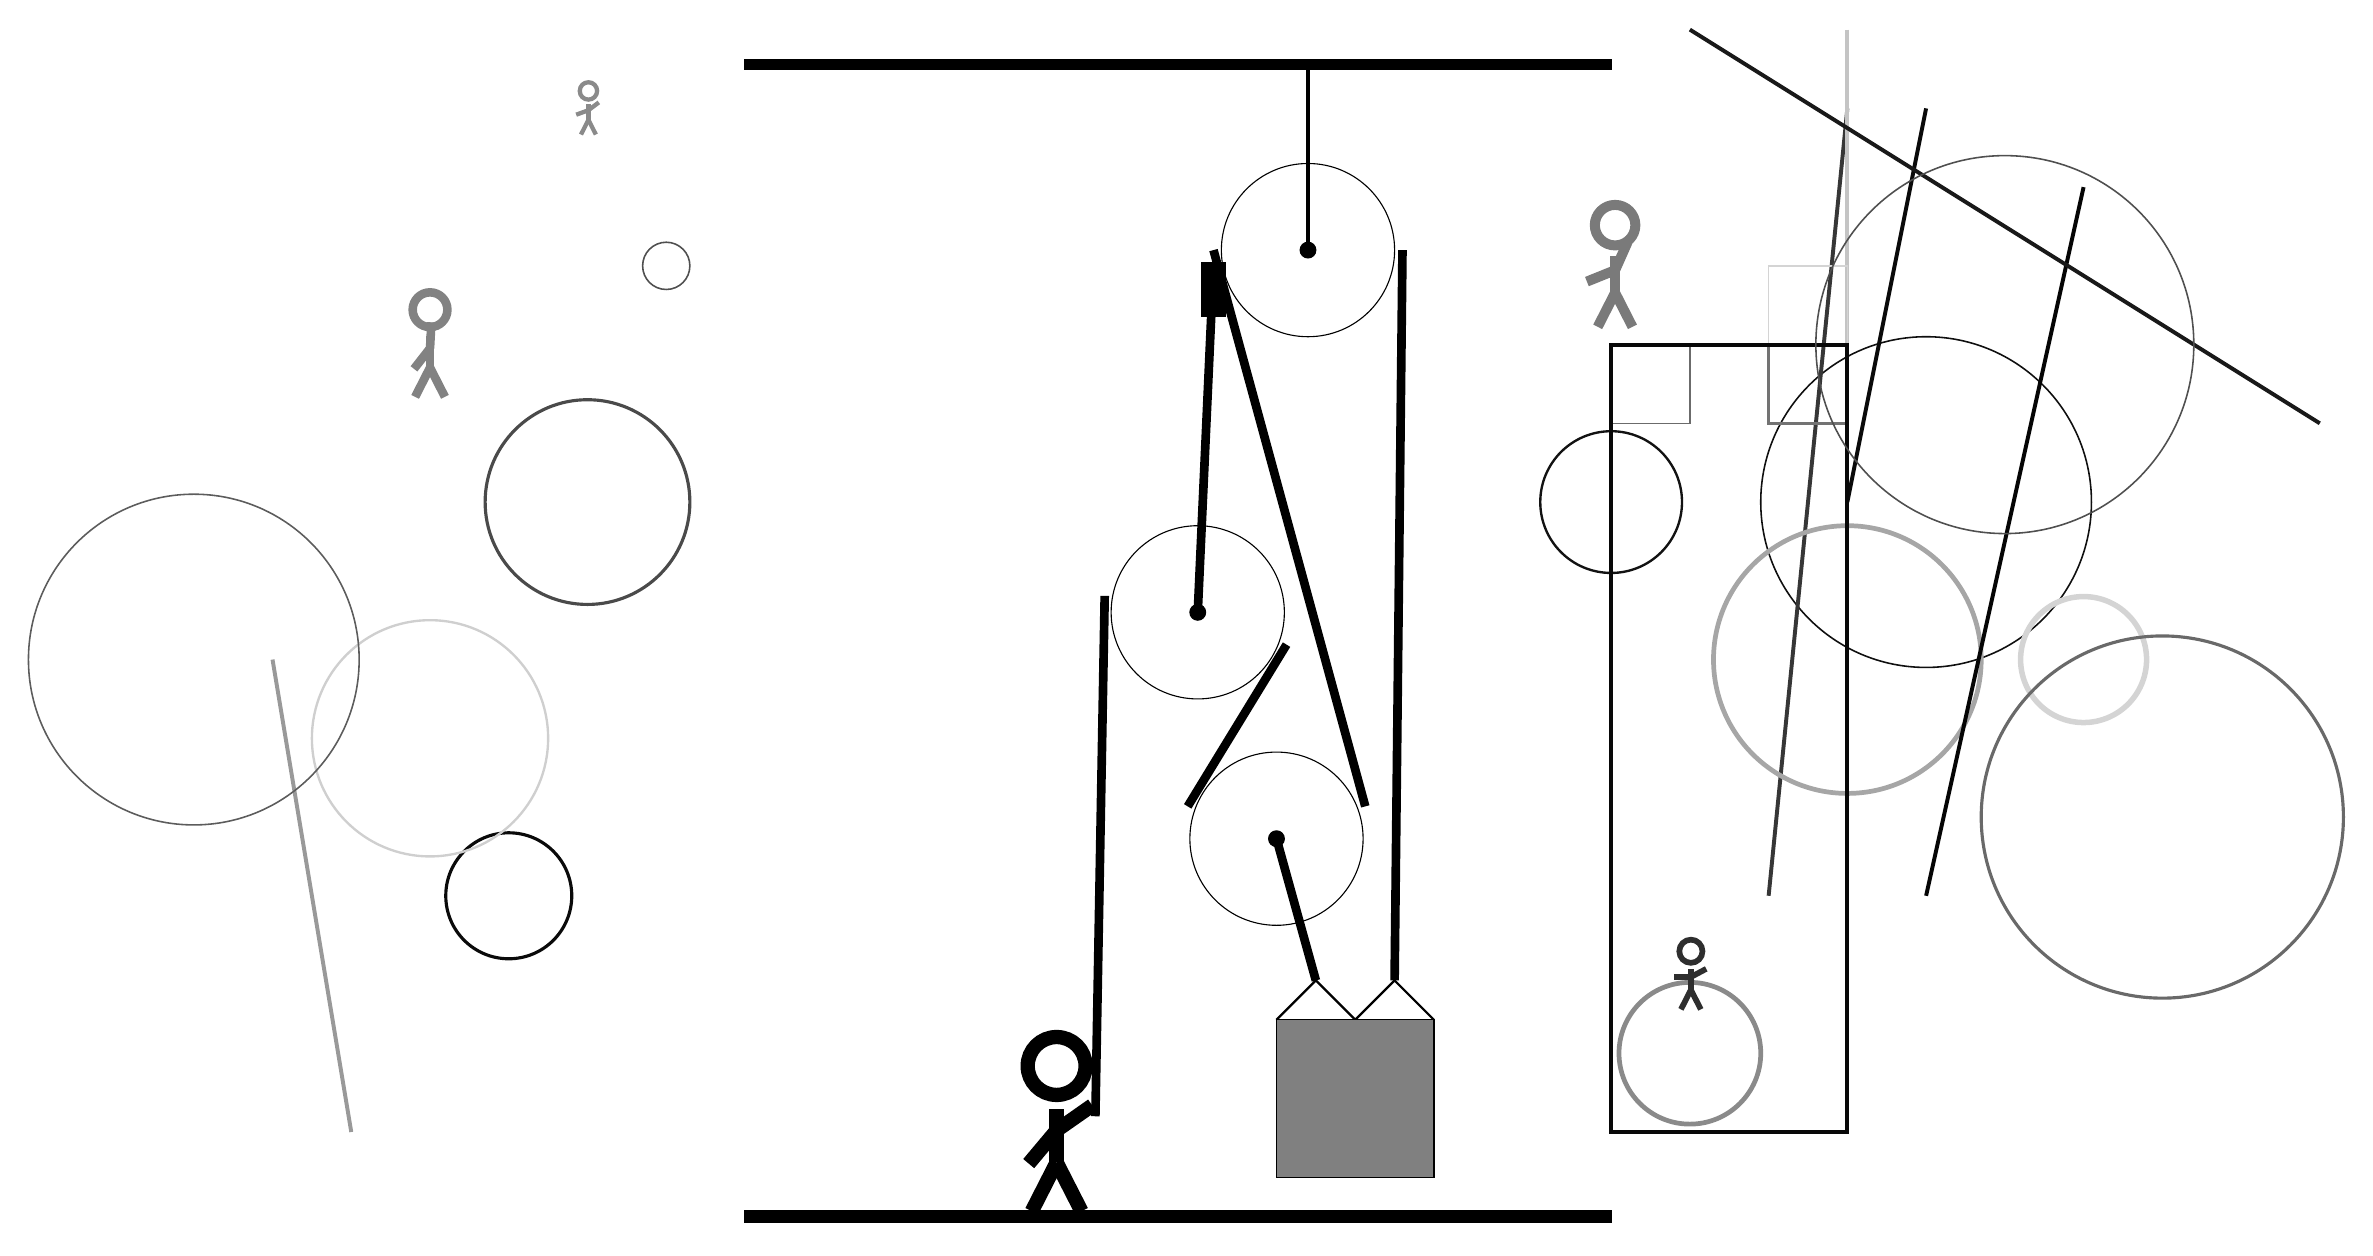
\begin{tikzpicture}
			%%%%% START %%%%%
			
			\draw[fill=black] (-6, 11.5) rectangle (5, 11.625);
			
			\draw (-0.25, 4.6) circle (1.1);
			\draw[fill=black] (-0.25, 4.6) circle (0.1);
			
			\draw (0.75, 1.725) circle (1.1);
			\draw[fill=black] (0.75, 1.725) circle (0.1);
			
			\draw (1.15, 9.2) circle (1.1);
			\draw[fill=black] (1.15, 9.2) circle (0.1);
			\draw[very thick] (1.15, 9.2) -- (1.15, 11.5);
			
			\draw[thick]  (0.75, -0.575) -- (1.25, -0.075) -- (1.75, -0.575) -- (2.25, -0.075) -- (2.75, -0.575);
			\draw[fill=black!50] (0.75, -0.575) rectangle (2.75, -2.575);
			
			\draw [line width=0.4mm, color=black!71](-8, 6) circle (1.3);
			
			\draw [line width=0.2mm, color=black!69](-7, 9) circle (0.3);
			\draw [line width=0.2mm, color=black!94](9, 6) circle (2.1);
			\draw[line width=0.5mm, color=black!79](8, 11) -- (7, 1);
			\draw[line width=0.5mm, color=black!23](8, 12) -- (8, 8);
			\draw[line width=0.5mm, color=black!96](8, 6) -- (9, 11);
			\draw [line width=0.4mm, color=black!96](-9, 1) circle (0.8);
			\draw[line width=0.4mm, color=black!55] (7, 7) rectangle (8, 8);
			\draw[line width=0.2mm, color=black!17] (7, 9) rectangle (8, 8);
			\draw [line width=0.6mm, color=black!46](6, -1) circle (0.9);
			
			\node[line width=0.5mm, color=black!52] at (5, 9) {\Strichmaxerl[7][22][66]};
			\draw [line width=0.3mm, color=black!60](-8, 7) circle (0.0);
			\draw [line width=0.7mm, color=black!17](11, 4) circle (0.8);
			\draw [line width=0.6mm, color=black!35](8, 4) circle (1.7);
			\draw[line width=0.5mm, color=black!40](-11, -2) -- (-12, 4);
			\node[line width=0.3mm, color=black!49] at (-10, 8) {\Strichmaxerl[6][52][87]};
			
			\draw[line width=0.2mm, color=black!58] (5, 8) rectangle (6, 7);
			\draw [line width=0.4mm, color=black!59](12, 2) circle (2.3);
			\draw [line width=0.3mm, color=black!19](-10, 3) circle (1.5);
			
			\draw[line width=0.5mm, color=black!98](9, 1) -- (11, 10);
			\draw [line width=0.2mm, color=black!64](-13, 4) circle (2.1);
			\node[line width=0.7mm, color=black!82] at (6, 0) {\Strichmaxerl[4][0][28]};
			
			\node[line width=0.5mm, color=black!46] at (-8, 11) {\Strichmaxerl[3][20][37]};
			\draw [line width=0.3mm, color=black!93](5, 6) circle (0.9);
			\draw[line width=0.5mm, color=black!97] (5, -2) rectangle (8, 8);
			
			\draw[line width=0.5mm, color=black!90](6, 12) -- (14, 7);
			\draw [line width=0.2mm, color=black!69](10, 8) circle (2.4);
			
			\draw[line width=1.1mm] (-0.25, 4.6) -- (-0.05, 9.0);
			\draw[line width=1.1mm, fill=black](-0.15, 8.4) rectangle (0.05, 9.0);
			\draw[line width=1.1mm] (-1.55, -1.8) -- (-1.4318, 4.8083);
			\centerarc[line width=1.1mm](-0.25, 4.6)(-20:170:1.2000000000000002);
			\draw[line width=1.1mm] (0.8776, 4.1896) -- (-0.3776, 2.1354);
			\centerarc[line width=1.1mm](0.75, 1.725)(160:380:1.2000000000000002);
			\draw[line width=1.1mm] (1.8776, 2.1354) -- (-0.05, 9.2);
			\draw[line width=1.1mm](0.75, 1.725) -- (1.25, -0.075);
			\centerarc[line width=1.1mm](1.15, 9.2)(0:180:1.2000000000000002);
			\draw[line width=1.1mm] (2.35, 9.2) -- (2.25, -0.075);
			
			\node at (-2, -1.9) {\Strichmaxerl[10][50][35]};
			
			\draw[fill=black] (-6, -3) rectangle (5, -3.15);
			
			%%%%% END %%%%%
		\end{tikzpicture}
	\end{figure}	
\end{document}